\documentclass{article}
\usepackage[english]{babel}
\usepackage{url}
\usepackage{graphicx}
\usepackage{amsthm}
\begin{document}
	\begin{titlepage}
		\centering
		{\scshape\Large INF142 submission one.\par}
		\vspace{3em}
		{{\scshape\large By Kristian Os \par}}
        \vspace{5em}
        
\includegraphics[scale=0.5]{uibLogo}
		\vfill
		\large\today
	\end{titlepage}
	\pagebreak
	\section{DNSSEC}
		\subsection{Definitions}
        \begin{itemize}
            \item DNS - Domain Name System
            \item DNSSEC - for Domain Name System Security Extensions.
            \item Root zone - This is the first node, DNS looks in the DNS hierarchy
            \item ZSK - Composed of a public key and a private key. Used to sign the fields in the area\cite{ovh}
            \item KSK - Composed of a public key and a private key. Used to sign the ZSK keys.\cite{ovh}
			\item ccTLD - Country code top-level domain, E.g .no, .se, .uk. 
            \item gTLD - Generic top-level domain, E.g .com, .org, .net
        \end{itemize}
		\subsection{What does DNS do?}
		For one node to reach another node on the Internet there must be denoted a number/name as an address. It must be unique so that one address only can point to one node. It might be looked at as the phone book of the Internet, where a telephone number are the ip-address and name are the domain name.
        This system is made out of many layers where each super-zone controls many sub-zones. \\
        \begin{figure}[htbp]
            \centering
            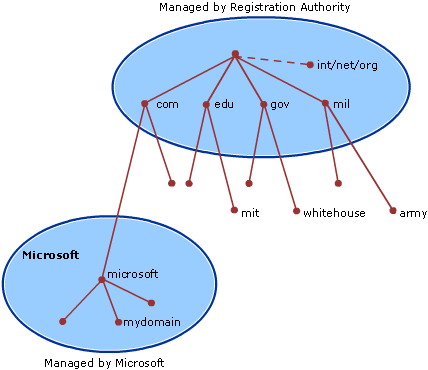
\includegraphics[scale=0.6]{dnsStruct}
            \caption{How the DNS zone layer is built up\cite{microsoftDnsModel}}
        \end{figure}\\
		There are many companies that manages these root DNS zone so that each node has one of these unique addresses. For the same reason as we do not reference our devices based on their MAC-addresses, DNS translates the name version of the address to a number. This makes it much easier to remember the different number versions of the address.
		\subsection{Security}
		Within the DNS there are no security measures that can stand to the modern attacks that are getting more complex and malicious by the day. Recently a vulnerabilities in the DNS were found that allowed an attacker to redirect a DNS lookup to retrieve a false IP-address. This way the user gets a fake version of the intended site and the attacker can steal information or manipulate messages/transactions for their own gain. However for this to work all domains that is registered must also implement DNSSEC on their own servers. This in turn requires the parent zones and TLD in question to have implemented DNSSEC as well.
	        \subsubsection{vulnerability? (Before DNSSEC)}
	        One DNS variant is DNS cache poisoning. For this exploit to work the attacker must get control of a DNS server and a DNS lookup must go through the poisoned DNS server. The attacker points an address like "www.uib.no" to a malicious IP-address. This way when a user types in "www.uib.no" he gets redirected to the malicious version of the site that the attacker owns.\cite{bellovin}
	        \subsubsection{After the implementation of DNSSEC}
	        With the implementation of DNSSEC organisations like UIB, Google and even the big tech leaders that controls the big nodes can sign the DNS records using public-key cryptography\cite{icann}
	        Now that each DNS server is signed with one of these keys the browsers know when a server is compromised and can select another one that is trusted.\\
	        \begin{figure}[htbp]
	        	\centering
	        	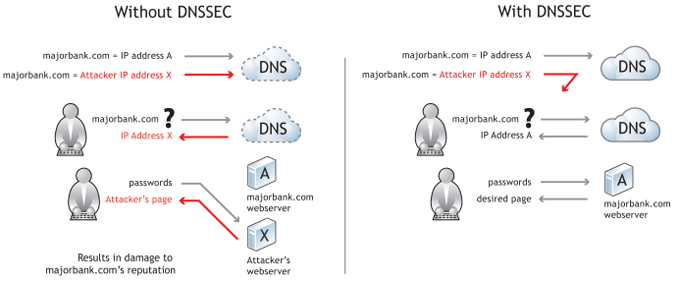
\includegraphics[width=1.0\textwidth]{dnsVsDnssec}
	        	\caption{Demonstrating DNSSEC on a theoretical plane.\cite{icannDnssec}}
	        \end{figure}
				\paragraph{Keys - KSK and ZSK}
				KSK is a long term key and ZSK is a short term key. For the root zone these keys are generated at different intervals. These events are called "Root KSK Ceremonies" and here the KSK is used to sign a set of ZSKs that will be used to sign the DNS root zone for three months until the next new ceremony. \cite{iana}
		\subsection{How does this help the average user}
		For every TLD/domain/zone that implements DNSSEC the Internet becomes a little more safe to use. However there are many people who use the Internet today that may not have the expertise to show enough caution to defend against DNS attacks. There are also people that does not have the knowledge to recognise the many dangers of the Internet. These people will only have to hope that the site they use as a bank or their favourite shopping site does implement DNSSEC before their information gets redirected. 
		\subsection{A brief history of DNS and DNSSEC}  
		DNS was not implemented until a computer scientist Paul Mockapetris started the first DNS server in 1983. Before then everyone had to remember the relative IP-addresses which of course was very inconvenient and hard to do if you needed to keep track of many sites.
		It became an internet standard in 1986 and eventually caught on in the year 1988.
		This worked very well for two years until a computer scientist named Steven Bellovin discovered a major flaw in the DNS protocol. It was actually made a secret until 1995 when Internet Engineering Task Force(IETF) begins discussing implementation of a security addition to DNS.
		The fist capable version of DNSSEC was finished in 1999, but with a lot of remodelling and tests, the version that stood finished for zone implementation was done.
		The first zone to enable DNSSEC was Sweden, making .SE the first ccTLD to enable DNSSEC in march 2005.\cite{NLnetLabs}
		\subsection{In debt development of the DNSSEC}
		Discussing from the point Sweden implemented DNSSEC into their ccTLD to date the technology has gone through a lot. In 2007 Automated updates of DNS security Trust Anchors was implemented.\cite{trustAnchor} 
		Before this it the DNSSEC signatures normally came from the operating system or other trusted sources. Now it was possible to update the DNSSEC signature at intervals so that the even cracking a key made it useless after a new key was generated, implemented and updated.\cite{icann} It was only in 2010 the first generic TLD was first signed. This was the .org domain and the root zone was signed later that year. Signing a TLD gave a massive boost in the promotion of DNSSEC deployment which is essential for the system to work. Also this is when the first KSK key ceremony ever. The next gTLD that implemented support for DNSSEC was .com only march the next year and in 2012 the number of signed TLDs was over 90.\cite{verisign}\\ At the start of 2015 there where 789 TLDs in the root zone in total, 615 had signed and 604 have trust anchors published as records in the root zone.\cite{icannStats} This is a tremendous growth when we look back to the early days of DNSSEC and how few TLDs that had signed only in 2010.
        \subsection{Where are we now}
		DNSSEC has only grown these past years and will hopefully grow even more. with a continue to grow even more in the future with a hope that all TLDs implement DNSSEC and to have trust anchors in the root zone. The current numbers give that 1502 are in the root zone in total, 1354 signed and 1342 have trust anchors in the root zone.\cite{icannStats}
		\subsection{Conclusion}
		While the implementation of DNSSEC does increase the authentication and integrity of DNS responses, it also takes a far bit more to actually implement it for each domain. As it stands when there are so many TLDs that have signed and implemented trust anchors in the root zone, we can only look forward and hope that all TLDs implement DNSSEC, so all domains have the choice at least to implement DNSSEC into their server.
	    There will always be dangers on the Internet, but we should do what we can not to make it easy for those who want to harm the Internet
	\section{Two-factor authentication}
        \subsection{Generation}
    	There are many different ways of generating a one-time password(OTP). Here it will be discussed some methods of generating a OTP and how they are used. For a password to be considered a OTP it must only be valid for one login session or transaction. 
    		\subsection{Time-synchronized}
            One method of generating and distributing such password is to give each user a personal token that, when used, gives a one time password. In the device an precise clock that is synchronised with the clock on the authentication server. With these OTP time is a very big factor in the generation of passwords. The password algorithm is given the current time rather than, or with the previous password or a key.One downside is the stability of clocks. If the clock in the token gets out of sync for whatever reason, this will fail since it will generate two different OTPs. If correct this OTP is only valid for a specific length after it has been generated. This method may generate a key on a variety of devices such as a mobile phone, mobile device running software or a proprietary device. 
            \subsection{Mathematical algorithms}
            One other branch of generating OTPs would be to generate from a purely mathematical point. Here one method would be to have a counter in both the authenticator and the generator. 
            This way if the seed number(counter) is 04203 in both devices and they use an algorithm to calculate an OTP. This removes the risk of de-synchronisation and can give very powerful codes that is near impossible to crack.
            Another version would be a hash chain. This requires a starting value and a hash function. This hash function may be of any implementation. Then only one more thing is needed, to hash the starting value many times. For example one could hash the seed 1000 times, insert that into the authenticator and when the user logs in he user a OTP that has hashed 999 times. This way the authenticator only needs to hash the OTP one time and compare it with the stored value that was hashed 1000 times beforehand. Now that the action was successful the authenticator stores the new value and it repeats until it needs to be reset for safety reasons.\cite{OTP-system}
            This hash function is one-way so anyone who manages to snap up a OTP and tries to "de-hash" it does not get the next OTP. Only some other value.
        \subsection{Distribution}
        The act of making sure that the OTP gets to the user in a fast, secure and convenient method.
            \subsubsection{Text messages}
            One very common technology for distribute OPTs is by text messages. This is has a very low implementation cost and is available to most mobile devices and trough text-to-speech conversion, all telephone devices either land-line or mobile.
            One drawback of this is the users cost of receiving each OTP and the fact that many of these passwords does not get encrypted very well. Also the delay from login initialization to login success can be a significant factor when customers choose a service.
            \subsubsection{Mobile Application} 	
            Many companies that has services that require authentication has started developing applications where you generate new codes all the time and last only for 20-30 seconds. This way there is constant change in the available OTP
            \subsubsection{Hard-copy}
            Some countries on-line banking systems have developed a system that is based on the order a set of OTPs has to be used. The bank sends the user a sheet of paper where the OTPs are hidden by a layer similar to scratch tickets at lotteries. Then when a user wants to login the user only has to scratch away the next OTP in the given order and use that. Making it so that it is just "generated" when in reality it was generated a long time ago. One big drawback of this is that it takes a very long time for the user to get his OTPs when the user starts or runs out of codes.
    \subsection{Conclusion}
    As described above there are quite a few ways of doing proper authentication by OTP and they all have their pros and cons. Thinking that one is a lot better than the others or that one is really bad will just lead to a stagnation in development of a technology that will dominate the authentication methods. The pursuit for faster, safer and overall better authentication should and will always be the goal for researchers and developers.
			
		
        
    \clearpage
	\nocite{*}
	\bibliography{mainBib}
	\bibliographystyle{plain}

\end{document}